\documentclass[sigconf,review,anonymous]{acmart}

\usepackage{tikz}
\usetikzlibrary{positioning,arrows.meta,fit}

\AtBeginDocument{%
  \providecommand\BibTeX{{Bib\TeX}}}

\setcopyright{none}
\copyrightyear{2026}
\acmYear{2026}
\acmDOI{}
\acmConference[ICAIF '26]{ACM International Conference on AI in Finance}{2026}{}
\acmISBN{}

\begin{document}

\title{Learning Conditional TP2 Violation Opportunities in SPY American Call Options}

\author{Anonymous Author(s)}
\affiliation{%
  \institution{Anonymous Institution}
  \country{}}

\renewcommand{\shortauthors}{Anonymous et al.}

\begin{abstract}
We study whether machine learning can identify economically meaningful total-positivity-inspired (TP2) violations in the SPY American call option surface. From conservative bid/ask TP2 violation episodes, we construct strategy-level labels for the two structurally viable call strategies, T1 and K2, using leakage-safe rolling train, validation, and test splits over 2014--2026 (2013 excluded as a data-vendor anomaly). The prediction task is not to detect TP2 violations, but to decide which episode-strategy pairs are worth trading.

Under a \$1,000 normalized exposure convention, trading every T1/K2 episode unconditionally over the 2021--2026 out-of-sample test years loses \$12.52M (Sharpe $-1.01$, 2 of 6 years profitable). Three independent learned selectors -- a LightGBM classifier, a feedforward network (MLP) on a 48-feature dictionary, and a TP2-MV-ALiBi transformer with multivariate ALiBi attention over historical episodes -- convert this into a positive out-of-sample portfolio under an identical, fully causal selection rule: trade whenever the calibrated model's probability is at least 0.5, with no other tuning. Single-model results range from Sharpe 1.25 (LightGBM) to 2.60 (MLP) to 1.51 (transformer); a 5-seed transformer ensemble reaches Sharpe 2.36 with 6 of 6 years profitable and the smallest drawdown of any model tested. We report a methodological finding explicitly: comparing a single MLP fit against a multi-seed transformer ensemble is not a controlled comparison, and correcting for it reverses which model appears superior -- ensembling improves the transformer (Sharpe 1.51 to 2.36) but degrades the MLP (2.60 to 1.66) -- and the underlying single-model gap between the two is not statistically significant at six test years. We additionally compare our results to a published SPX TP2-violation trading study using an identical per-trade return convention and find a large, unexplained gap in realized magnitude between the two underlyings.
\end{abstract}

\begin{CCSXML}
<ccs2012>
 <concept>
  <concept_id>10010147.10010257.10010258.10010259</concept_id>
  <concept_desc>Computing methodologies~Machine learning</concept_desc>
  <concept_significance>500</concept_significance>
 </concept>
 <concept>
  <concept_id>10010405.10010481.10010485</concept_id>
  <concept_desc>Applied computing~Economics</concept_desc>
  <concept_significance>300</concept_significance>
 </concept>
</ccs2012>
\end{CCSXML}

\ccsdesc[500]{Computing methodologies~Machine learning}
\ccsdesc[300]{Applied computing~Economics}

\keywords{options, total positivity, machine learning, transformer, SPY, statistical arbitrage}

\maketitle

\section{Introduction}
\label{sec:intro}

Option prices across strikes and maturities are not arbitrary. No-arbitrage theory imposes shape restrictions on the option surface, and violations of these restrictions can indicate relative-value opportunities or market frictions. One such structure is total positivity of order two (TP2), which implies multiplicative inequalities between option prices arranged across strike and maturity. Prior work links TP2 violations to option-market arbitrage strategies in theory, but detecting a violation is not the same as constructing a profitable, tradable strategy: bid/ask spreads, liquidity, stale quotes, early expiration, and regime changes can all turn a theoretical violation into an unprofitable trade in practice.

This paper studies TP2-inspired violations in SPY American call options. SPY is highly liquid, widely traded, and has a dense option surface across strikes and expirations. Although SPY options are American-style, the terminal payoff of a call at expiration is still $\max(S_T-K,0)$, which makes expiration-payoff accounting a clean way to study the economic content of TP2 violations while still requiring care around execution assumptions, dividends, and early assignment of short call positions.

Our central question is whether machine learning can distinguish profitable TP2 violation episodes from unprofitable ones using only information available at the violation date. We do not frame the task as violation detection; we first construct TP2 episodes and then ask whether a model should trade the T1 strategy, trade the K2 strategy, or skip the episode. This framing matters because unconditional trading is not profitable: over the 2021--2026 out-of-sample test years, trading every valid T1/K2 expiration-payoff episode under a \$1,000 normalized exposure convention loses \$12.52M in aggregate (Sharpe $-1.01$, only 2 of 6 years profitable). The research problem is therefore one of conditional selection, not detection.

We evaluate three independent selectors under rolling walk-forward out-of-sample splits, each training on three years, calibrating on the following validation year, and testing once on the next year, so that no test-year information ever enters training or calibration. Our baselines are a LightGBM classifier and an MLP, both trained on a common 48-feature selected dictionary. We then introduce a TP2-MV-ALiBi transformer that attends to historical TP2 episodes using a multivariate attention bias over five domain-relevant distances: time, option-surface location, short-leg structure, liquidity, and lifecycle stage.

A methodological contribution of this paper, separate from the modeling results, concerns trade selection. An earlier iteration of this pipeline selected trades via a validation-tuned probability threshold or a rank-based selection fraction; on inspection, both were prone to overfitting a single validation year, and the fraction rule was additionally non-causal, since its cutoff depended on the full test period's prediction distribution rather than information available at trade time. We replace both with the simplest rule available: trust the calibrated model directly, trading whenever its predicted probability is at least 0.5 and skipping otherwise, with no tuning of any kind. This rule is fixed a priori as the natural decision boundary for a calibrated binary probability, not chosen from any data; as a diagnostic, we separately confirm it behaves consistently across the early and late halves of the test period rather than being an artifact of one favorable stretch (Section~\ref{sec:calibration}).

We also identify and correct a comparison bias that is easy to introduce unintentionally: naively comparing a single model fit for one architecture against a multi-seed ensemble for another architecture favors whichever happens to have been ensembled, independent of which architecture is actually better. Controlling for this by testing both architectures at matched seed counts changes which model appears superior in our results, and the underlying single-model gap between them is not statistically significant given six test years. We report this finding directly rather than presenting only the comparison that favors the transformer architecture we introduce.

The contributions of this paper are threefold. First, we construct a leakage-safe TP2 episode pipeline for SPY American call options with explicit strategy-level labels, transaction-cost-aware realized returns, and a documented, causal trade-selection rule. Second, we compare unconditional trading, tree-based selection, MLP selection, and a TP2-specific multivariate ALiBi transformer under an identical rolling evaluation protocol, selection rule, and metric set. Third, we identify a model-comparison confound related to ensembling and report the controlled, corrected comparison, and we benchmark our results directly against a published SPX study of the same underlying phenomenon.

\section{Background and Related Work}
\label{sec:related}

\subsection{TP2 Inequalities and Options Arbitrage}
Total positivity of order 2 (TP2) is a shape restriction on call option prices arranged across strike and maturity: under the Black--Scholes model, and more generally a broad class of arbitrage-free pricing models, the ratio of a higher-strike call price to a lower-strike call price at the same maturity increases with time-to-expiry~\cite{glasserman2026tp2theory,glasserman2023convexity}. A TP2 violation is a stronger condition than the absence of calendar-spread arbitrage and can indicate a relative-value trading opportunity when it occurs empirically. Our episode-detection logic and normalized-exposure trading convention follow the empirical framework of a companion study of TP2-violation trading strategies on S\&P 500 index (SPX) options~\cite{glasserman2025tp2}, which finds that TP2 violations are rare, typically reverse quickly, and can be traded profitably on both an absolute and risk-adjusted basis. We adopt that study's per-trade normalized-return convention directly in Section~\ref{sec:spx-benchmark} to make a like-for-like comparison against our SPY results possible. The theoretical TP2 property itself~\cite{glasserman2026tp2theory} is established for European-style, cash-settled index option prices; SPY options are American-style with dividend-paying underlying shares, so early exercise and dividend timing are institutional features of our setting that the theory does not need to address~\cite{cosma2020earlyexercise}. We return to the implications of this gap in Section~\ref{sec:limitations}.

\subsection{Machine Learning for Options}
Machine learning applied to options has largely targeted implied-volatility surface fitting, delta-hedging, and derivative pricing. A separate line of work applies machine learning directly to trading and market-making decisions under realistic execution constraints, including bid-ask spreads and order-book dynamics~\cite{kearns2013mlmicrostructure}. Our setup differs from both: rather than forecasting a continuous quantity such as implied volatility, we pose a binary trade/no-trade classification problem conditioned on an already-detected TP2 violation, and, following the market-microstructure-aware tradition of the latter line of work, we evaluate models purely on realized, cost-aware trading performance under rolling out-of-sample walk-forward splits rather than on a pricing-error metric.

\subsection{Attention with Linear Biases}
ALiBi~\cite{press2022alibi} replaces learned or sinusoidal positional embeddings in transformer attention with a fixed linear penalty on attention logits, proportional to the distance between query and key positions, using a per-head slope fixed at initialization. This is effective for extrapolating to longer sequences in language modeling, where the relevant notion of distance is scalar token position. That notion of distance is not directly meaningful for TP2 episodes, which are better characterized by several simultaneous, domain-relevant distances rather than one. Our architecture, described in Section~\ref{sec:transformer}, replaces ALiBi's single scalar distance and fixed slope with a five-dimensional distance vector and a slope that is learned, rather than fixed, separately per distance type and per attention head.

\section{Data and Episode Construction}
\label{sec:data}

\subsection{Data Source and Scope}
\label{sec:data-source}
We use SPY American call options from 2014--2026. The year 2013 is excluded: the data vendor reports 49{,}090 episodes in 2013 versus 438 in 2014, a discontinuity consistent with a vendor-side data-quality anomaly rather than a genuine change in market structure. After filtering to the T1/K2 strategy universe described below, our dataset contains 177{,}487 unique episodes, spanning 2014-02-03 to 2026-06-04.

\subsection{TP2 Episode Detection}
A TP2 episode begins when a conservative bid/ask option-price rectangle violates the TP2 inequality $C(K_1,T_1)\cdot C(K_2,T_2) < C(K_1^{\ast},T_2)\cdot C(K_2^{\ast},T_1)$ for strikes $K_1 < K_2$ and maturities $T_1 < T_2$, using rounded-up adjusted strikes $K_1^{\ast}, K_2^{\ast}$ where an exactly matching strike is unavailable. We additionally remove any candidate pair that violates a vertical or calendar-spread no-arbitrage condition, so that trading profit cannot be attributed to an arbitrage artifact in the underlying price data rather than a genuine TP2 violation.

\subsection{Episode Tracking}
\label{sec:episode-tracking}
The raw detector output described above is daily and rectangle-level: the same economic TP2 violation, identified by its strike/maturity pair, can appear on multiple consecutive trading days. Treating every daily row as an independent observation would inflate the effective sample size and make the train/validation/test splits in Section~\ref{sec:method} harder to defend, since consecutive days of the same underlying violation are not independent events. We track episodes rather than daily rows: consecutive daily appearances of the same strike/maturity pair are grouped into a single pair episode, keyed on the pair's near-leg strike and maturity, with the four-leg rectangle (including rounded adjusted strikes) tracked as a diagnostic rather than part of the key, since forward and rounding adjustments can shift within the same economic episode.

Over the full raw detection history, 2{,}430{,}220 daily violation rows collapse to 2{,}098{,}213 pair episodes. Episode duration is heavily right-skewed: 88.66\% of episodes are single-session events, the median duration is one session, and the maximum observed duration is 14 sessions. Of these raw pair episodes, 50.6\% end in true reversion (the TP2 inequality resolves) rather than expiring, losing a required leg, or failing a liquidity filter. This raw population is prior to the conservative bid/ask filter, the T1/K2 restriction, and the cost-aware labeling described below; the T1/K2 episode count used for modeling throughout the rest of this paper (177{,}487 episodes, Section~\ref{sec:data-source}) is a downstream, filtered subset of it.

To track each episode beyond just its start, we build a lifecycle panel that follows every conservative TP2 episode across a fixed event-time window: a 20-session pre-event lookback through expiration, indexed relative to the first violation day (event day 0). Figure~\ref{fig:lifecyclepath} plots the resulting lifecycle path of normalized TP2 pressure -- the median and 10--90/25--75 percentile bands of the (rectangle-implied) pressure at each event day, across every tracked episode. Pressure is flat and slightly negative in the pre-event window, spikes sharply at day 0 by construction (the violation event itself), decays back toward zero over the following sessions, and drifts downward again as episodes approach the far end of the tracked window. This single panel is what makes the earlier reversion and duration statistics auditable: rather than only reporting summary counts, the underlying pressure trajectory that produces them is directly visible from pre-event lookback through to expiration.

\begin{figure}[t]
\centering
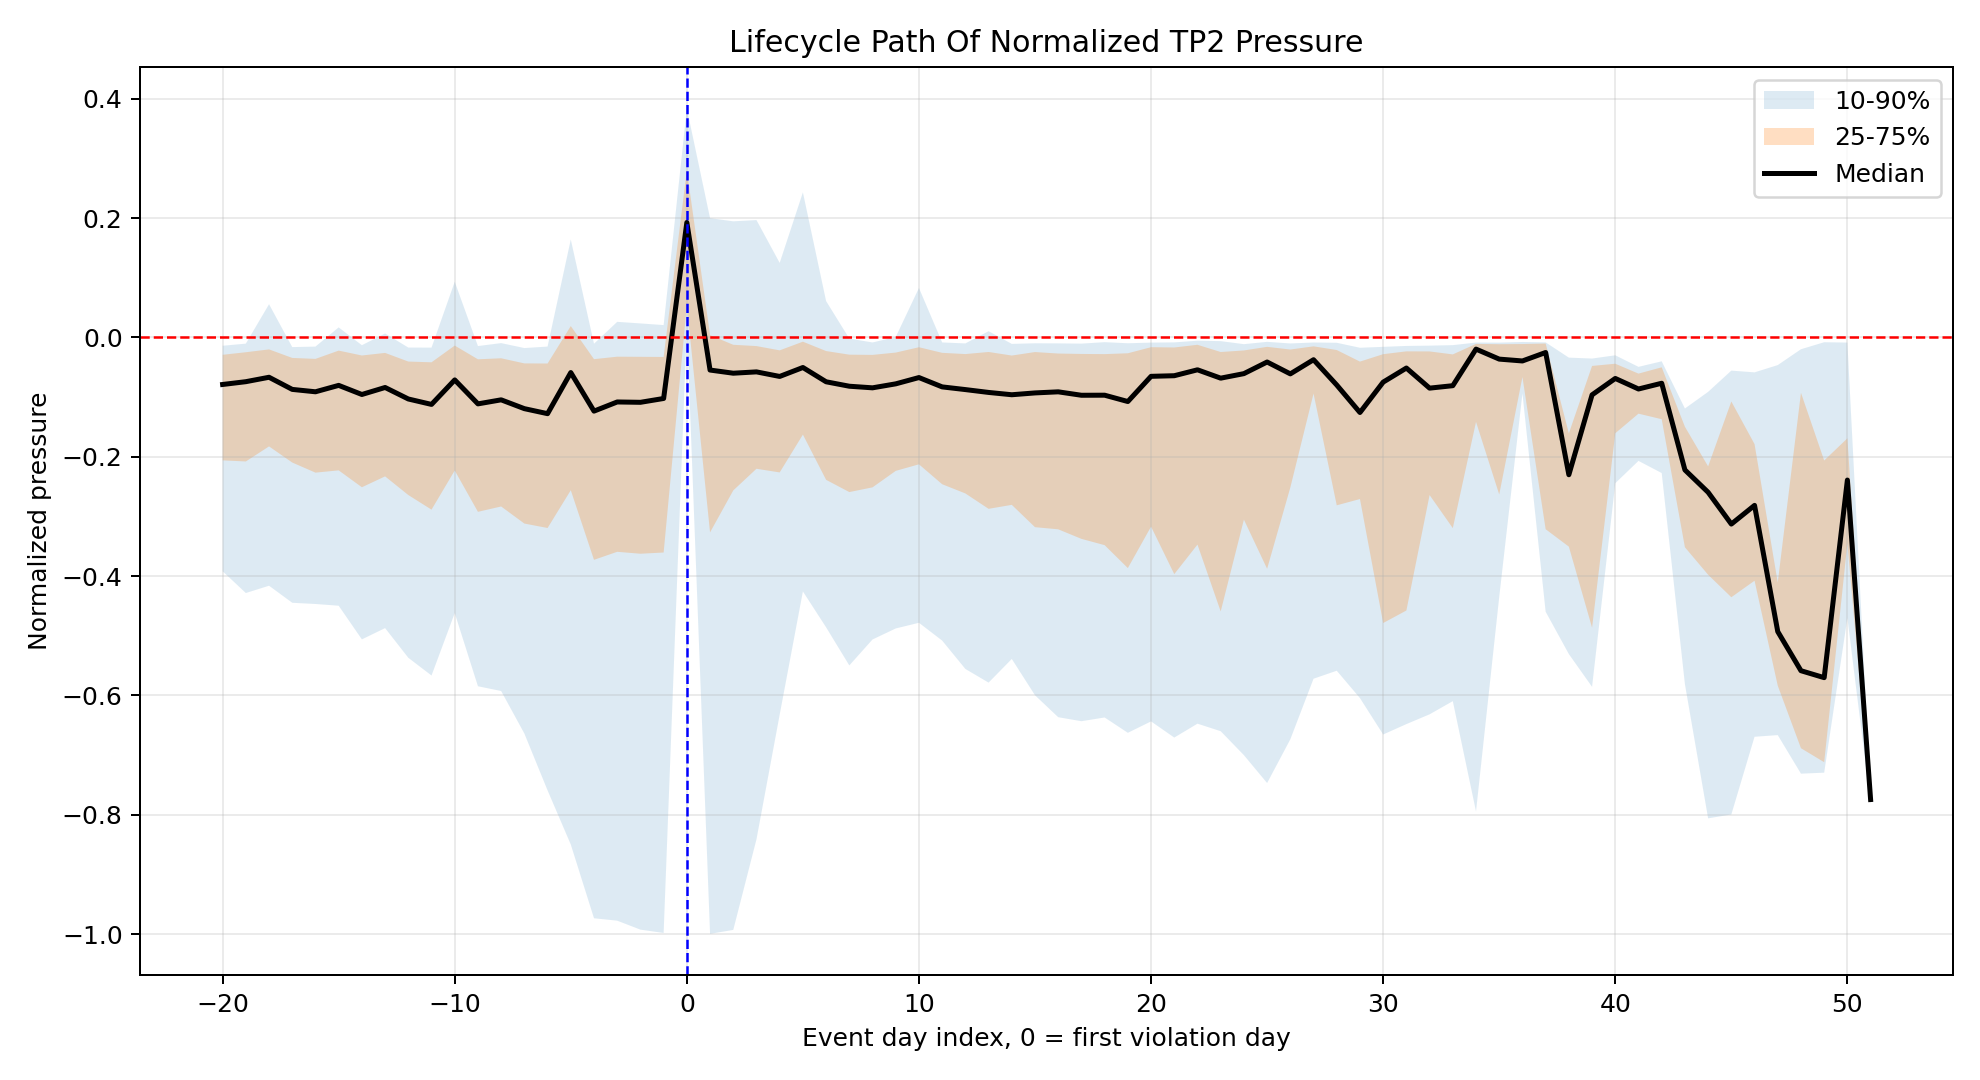
\includegraphics[width=\linewidth]{figures/lifecycle_normalized_pressure_band.png}
\caption{Lifecycle path of normalized TP2 pressure, event day $-20$ (pre-event lookback) through expiration. The dashed vertical line marks the first violation day (event day 0); shaded bands are the 10--90 and 25--75 percentile range across all tracked episodes.}
\label{fig:lifecyclepath}
\end{figure}

\subsection{Label Construction and Transaction Costs}
\label{sec:labels}
The primary label policy used throughout this paper holds positions to expiration and uses the terminal intrinsic payoff for the selected leg. Our realized-return calculation is cost-aware rather than a naive mid-price backtest: the entry leg of every trade is executed at the full bid-ask spread (long positions buy at the ask, short positions sell at the bid), and a commission of \$0.65 per contract is charged per leg, matching Interactive Brokers' published IBKR Lite fixed-rate US options commission.\footnote{\url{https://www.interactivebrokers.com/en/pricing/commissions-options.php}, accessed 2026.} Realized return is normalized by the trade's own gross exposure and then expressed in dollar terms via a \$1{,}000 fixed-exposure convention, so that a trade's normalized profit and loss is directly interpretable as a percentage return regardless of the underlying option's actual price level. This normalization matters in our data: raw, un-normalized exposures range from a median of \$7--\$11 to a maximum of \$814{,}000 per trade, which would make raw dollar comparisons across trades meaningless without it.

\subsection{Strategy Restriction: T1 and K2}
We restrict to the T1 and K2 strategy denominations, both of which short the shorter-dated leg of the TP2 violation. This is a structural prior decided on theoretical grounds before any model training: the two excluded denominations, T2 and K1, both short the longer-dated leg, exposing the position to a longer horizon over which an adverse market move can develop. We test this prior empirically rather than only asserting it theoretically: Section~\ref{sec:lgbm-scope} trains an unrestricted four-strategy classifier and shows that T2 and K1 lose heavily, consistent with the structural argument.

\section{Methodology}
\label{sec:method}

Figure~\ref{fig:pipeline} details the full pipeline described in this section, from raw SPY option quotes through the shared calibration and selection stage that produces the evaluated portfolio in Section~\ref{sec:results}.

\begin{figure*}[t]
\centering
\resizebox{0.86\textwidth}{!}{%
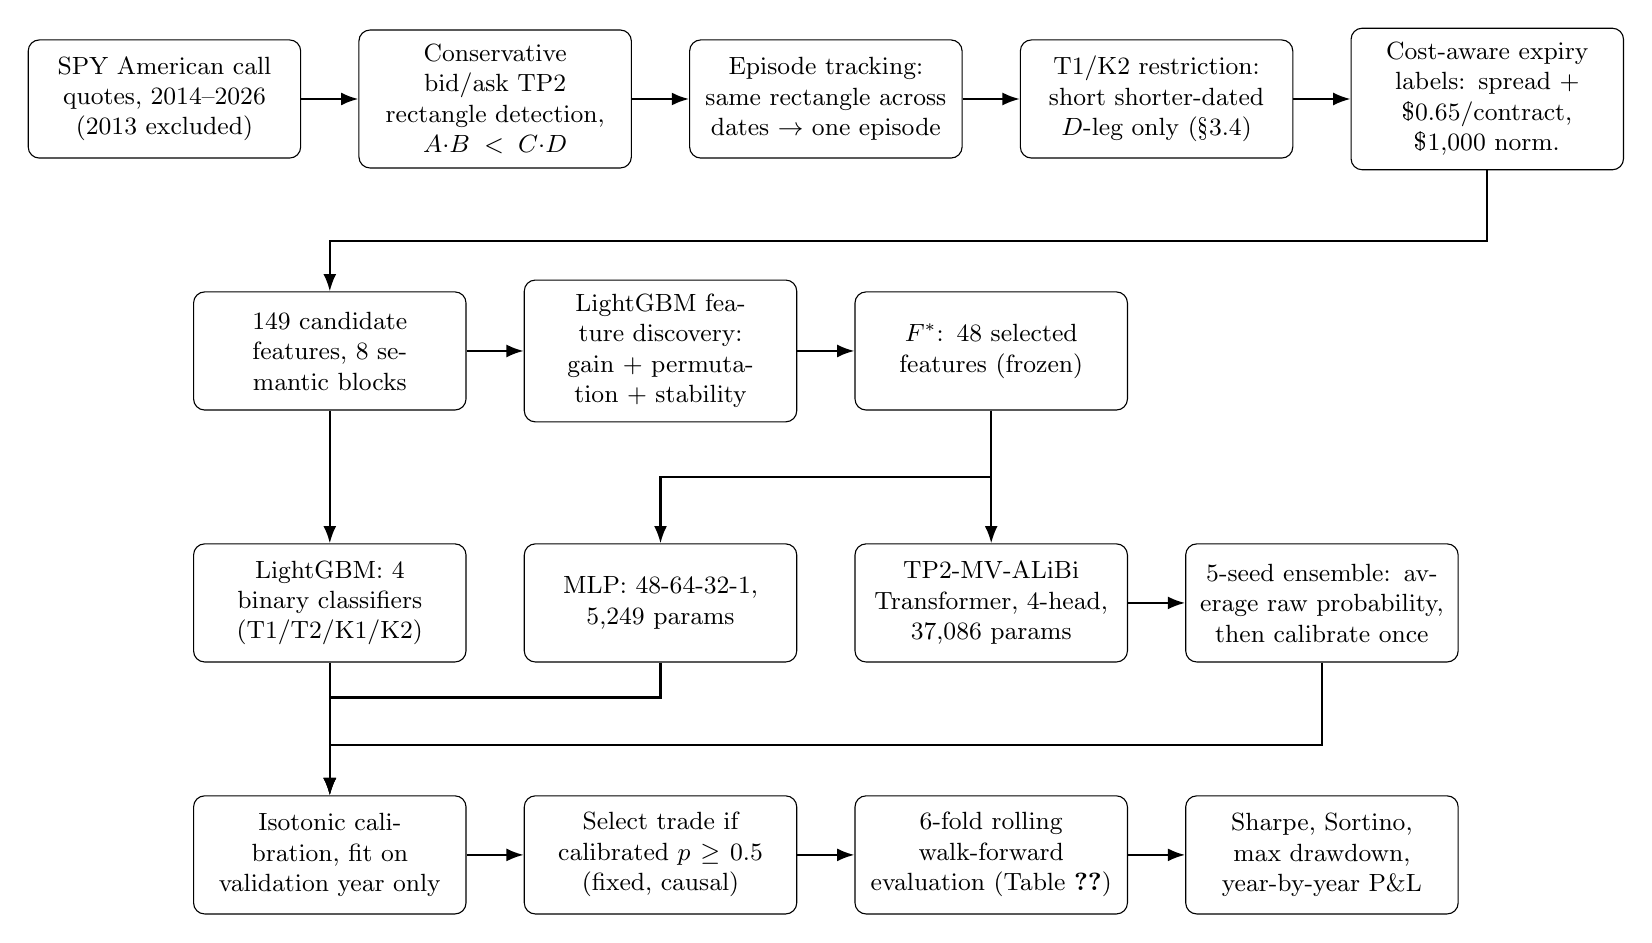
\begin{tikzpicture}[
  box/.style={draw, rounded corners, align=center, text width=3.1cm, minimum height=1.5cm, font=\small, inner sep=1.8mm},
  arr/.style={-{Latex[length=2.2mm]}, thick}
]

\node[box] (raw)      at (0,0)   {SPY American call quotes, 2014--2026 (2013 excluded)};
\node[box] (tp2)       at (4.2,0) {Conservative bid/ask TP2 rectangle detection, $A{\cdot}B < C{\cdot}D$};
\node[box] (episode)   at (8.4,0) {Episode tracking: same rectangle across dates $\to$ one episode};
\node[box] (restrict)  at (12.6,0){T1/K2 restriction: short shorter-dated $D$-leg only (\S3.4)};
\node[box] (labels)    at (16.8,0){Cost-aware expiry labels: spread + \$0.65/contract, \$1{,}000 norm.};

\node[box] (feat149)  at (2.1,-3.2)  {149 candidate features, 8 semantic blocks};
\node[box] (lgbmfs)   at (6.3,-3.2) {LightGBM feature discovery: gain + permutation + stability};
\node[box] (fstar)    at (10.5,-3.2) {$F^{\ast}$: 48 selected features (frozen)};

\node[box] (lgbm) at (2.1,-6.4)   {LightGBM: 4 binary classifiers (T1/T2/K1/K2)};
\node[box] (mlp)  at (6.3,-6.4)   {MLP: 48-64-32-1, 5{,}249 params};
\node[box] (tf)   at (10.5,-6.4)  {TP2-MV-ALiBi Transformer, 4-head, 37{,}086 params};
\node[box] (ens)  at (14.7,-6.4)  {5-seed ensemble: average raw probability, then calibrate once};

\node[box] (calib)  at (2.1,-9.6)  {Isotonic calibration, fit on validation year only};
\node[box] (select) at (6.3,-9.6)  {Select trade if calibrated $p \ge 0.5$ (fixed, causal)};
\node[box] (eval)   at (10.5,-9.6) {6-fold rolling walk-forward evaluation (Table~\ref{tab:folds})};
\node[box] (metrics) at (14.7,-9.6){Sharpe, Sortino, max drawdown, year-by-year P\&L};

\draw[arr] (raw) -- (tp2);
\draw[arr] (tp2) -- (episode);
\draw[arr] (episode) -- (restrict);
\draw[arr] (restrict) -- (labels);
\draw[arr] (labels) -- (16.8,-1.8) -- (2.1,-1.8) -- (feat149);
\draw[arr] (feat149) -- (lgbmfs);
\draw[arr] (lgbmfs) -- (fstar);
\draw[arr] (feat149) -- (lgbm);
\draw[arr] (fstar) -- (10.5,-4.8) -- (6.3,-4.8) -- (mlp);
\draw[arr] (fstar) -- (tf);
\draw[arr] (tf) -- (ens);
\draw[arr] (lgbm) -- (calib);
\draw[arr] (mlp) -- (6.3,-7.6) -- (2.1,-7.6) -- (calib);
\draw[arr] (ens) -- (14.7,-8.2) -- (2.1,-8.2) -- (calib);
\draw[arr] (calib) -- (select);
\draw[arr] (select) -- (eval);
\draw[arr] (eval) -- (metrics);
\end{tikzpicture}%
}
\caption{Detailed end-to-end pipeline. Top row: episode construction (Section~\ref{sec:data}). Second row: LightGBM-driven feature discovery reducing 149 candidate features to the frozen $F^{\ast}$ dictionary (Section~\ref{sec:method}.2). Third row: the three independently trained models -- LightGBM trains directly on the full 149-feature set (Section~\ref{sec:lgbm-scope}) and is additionally trained on all four strategy denominations to test the T1/K2 restriction; the MLP and transformer train on $F^{\ast}$ only; the transformer is evaluated both single-seed and as a 5-seed ensemble (Section~\ref{sec:seedcount}). Bottom row: one shared calibration, selection, and rolling-evaluation stage, so Section~\ref{sec:results} compares three scoring functions on identical downstream decisions rather than three different pipelines.}
\label{fig:pipeline}
\end{figure*}

\subsection{Rolling Evaluation Protocol}
We use a six-fold rolling walk-forward scheme with a three-year training window, a one-year validation year immediately following, and a one-year test year immediately following that, rolling forward one year at a time to cover test years 2021--2026 (Table~\ref{tab:folds}). No test-year information enters model training, probability calibration, or feature scaling for that fold: the feature scaler is fit on the training years only, and probability calibration (Section~\ref{sec:calibration}) is fit on the validation year only. We separately test an expanding-window alternative, where the training window grows to include all available history rather than a fixed three years, in Section~\ref{sec:window}.

\begin{table}[H]
\centering
\small
\begin{tabular}{lll}
\toprule
Train years & Validation year & Test year \\
\midrule
2017--2019 & 2020 & 2021 \\
2018--2020 & 2021 & 2022 \\
2019--2021 & 2022 & 2023 \\
2020--2022 & 2023 & 2024 \\
2021--2023 & 2024 & 2025 \\
2022--2024 & 2025 & 2026 \\
\bottomrule
\end{tabular}
\caption{Rolling walk-forward fold definitions.}
\label{tab:folds}
\end{table}

\subsection{Feature Selection}
We use LightGBM~\cite{ke2017lightgbm} as a feature-discovery tool, separate from its role as a trading model in Section~\ref{sec:lgbm-scope}. From 149 candidate features spanning eight semantic blocks (Table~\ref{tab:featureblocks}), we select 48 features, denoted $F^{\ast}$, using a composite importance score combining gain-based importance, permutation importance, and a temporal-stability penalty computed across folds. Only the selected feature values are passed to the MLP and transformer; LightGBM's own predictions, leaf indices, and importance scores are never used as model inputs downstream, so the comparison in Section~\ref{sec:results} is between three independent modeling approaches on a shared, inspectable feature set rather than a stacked ensemble.

\begin{table}[H]
\centering
\small
\begin{tabular}{lr}
\toprule
Feature block & Count in $F^{\ast}$ \\
\midrule
Market & 12 \\
Short-leg structure & 10 \\
Option risk & 10 \\
Surface location & 6 \\
Liquidity & 5 \\
TP2 geometry & 3 \\
Strategy and calendar & 1 \\
Lifecycle pressure & 1 \\
\midrule
Total & 48 \\
\bottomrule
\end{tabular}
\caption{Selected feature dictionary $F^{\ast}$ by semantic block.}
\label{tab:featureblocks}
\end{table}

\subsection{LightGBM Model}
\label{sec:lgbm-scope}
Our LightGBM model trains four independent binary classifiers, one per strategy denomination (T1, T2, K1, K2), each predicting whether that denomination's episode will be profitable. Unlike the MLP and transformer, LightGBM is trained on the full 149-candidate feature set, consistent with its role as a feature-discovery tool, and on all four strategy denominations, which lets us test the T1/K2 structural prior directly. We verified that LightGBM's T1 and K2 sub-models train and evaluate on an episode population identical to the MLP and transformer: 177{,}487 episodes for each strategy, with zero difference in the underlying episode-ID sets and matching base profitability rates (25.33\% for T1, 23.67\% for K2), so the model comparison in Section~\ref{sec:results} is not confounded by a different underlying data population despite LightGBM's broader candidate feature set.

\subsection{MLP Baseline}
The MLP baseline is a feedforward network with layer sizes 48, 64, 32, and 1 (ReLU activations, 5{,}249 parameters total), trained on the selected feature dictionary $F^{\ast}$. This model tests whether the selected features alone, without any sequence or historical-attention modeling, contain tradable signal.

\subsection{TP2-MV-ALiBi Transformer}
\label{sec:transformer}
Each candidate episode-strategy pair is encoded as a token combining its $F^{\ast}$ feature values, a strategy embedding, and calendar features. The current token attends to up to 64 prior episode tokens, drawn only from strictly earlier calendar days, via a single cross-attention block with four heads and hidden dimension 64 (37{,}086 parameters total, roughly seven times the size of the MLP baseline). The attention logit for head $h$ between the current token $i$ and a historical token $j$ is
\[
a_{ij}^{h} \;=\; \frac{q_i \cdot k_j}{\sqrt{d}} \;-\; m_h^{\top} d_{ij},
\]
where $d_{ij}$ is a five-dimensional vector of distances between episode $i$ and historical episode $j$ -- time elapsed, option-surface location, short-leg structure, liquidity, and lifecycle stage -- and $m_h$ is a learned, strictly positive per-head slope vector obtained via a softplus transform. This is the multivariate generalization of ALiBi's single scalar distance penalty described in Section~\ref{sec:related}. A same-strategy versus cross-strategy bonus term is added on top of the distance penalty. The model is trained with binary cross-entropy on the profitability label plus an auxiliary Huber-loss term on realized return, using AdamW with a learning rate of $3\times10^{-5}$, a linear warm-up over the first eight percent of training, a gradient clip norm of 1.0, and weight decay of $10^{-4}$. The model checkpoints on the epoch with the lowest validation loss rather than the epoch with the best validation ranking metric; an earlier iteration of this model checkpointed on the ranking metric, which allowed epochs with degrading calibration to be kept whenever ranking performance still appeared acceptable.

We verified the learned attention mechanism behaves as intended. Despite the five distance types spanning very different raw scales -- a mean scale near 4.9 for time elapsed versus near 0.66 for short-leg distance, roughly a seven-to-one ratio -- the learned slopes converge to a tight band of 0.26 to 0.27 across all five distance types. We checked this across every attention head and, in a 5-seed ensemble comprising 30 independently trained models across all folds and seeds, across every random initialization: the mean learned slope for each distance type falls between 0.262 and 0.266, with a standard deviation below 0.0035 in every case. The mechanism reliably compensates for the differing raw units across distance types rather than being dominated by whichever distance happens to have the largest raw magnitude.

\subsection{Probability Calibration and Trade Selection}
\label{sec:calibration}
For every model, we fit isotonic regression calibration~\cite{zadrozny2002transforming} on validation-year predictions and labels only, never on test-year labels, and apply the fitted calibration map unchanged to test-year predictions. For multi-seed ensembles, raw uncalibrated probabilities are averaged across seeds before calibration, and a single calibration map is fit on the averaged validation probabilities.

The trade-selection rule is a fixed decision with no tunable parameters: select any episode-strategy pair whose calibrated probability is at least 0.5, and skip otherwise. This rule depends on nothing but the current trade's own calibrated probability, so it is causal by construction and directly deployable. We evaluated two alternative rules during model development and rejected both. A validation-tuned absolute probability threshold, chosen by grid search to maximize raw validation-year profit and loss, was prone to selecting degenerate, near-minimal thresholds that chase rare large winners rather than reflecting genuine trade quality. A rank-based top-$K$ selection fraction, whose cutoff is re-derived as a quantile of the entire test period's prediction distribution, is non-causal: deciding whether to trade on a given date under this rule requires knowing the distribution of predictions over months that have not yet occurred relative to that date, which is not information available at trade time.

We use $p \ge 0.5$ because it is the natural decision boundary for a calibrated binary probability: under correct calibration, $p \ge 0.5$ is precisely the statement that a trade is more likely profitable than not, so the rule requires no tuning and no held-out data to define. It is fixed a priori, before any test-year result is examined, and is identical across every model and every fold. As a diagnostic rather than a selection procedure, we separately checked whether this fixed rule behaves consistently across the test period rather than being an artifact of one favorable stretch: split into an early half (2021--2023) and a late half (2024--2026) and scored on risk-adjusted metrics, both halves are solidly profitable under the identical, unmodified rule (Sharpe 1.17 and 2.88 respectively; 3 of 3 years profitable in each half), so the rule's behavior is not concentrated in one part of the evaluation window. This check does not inform the choice of rule and does not affect the six-year results reported in Section~\ref{sec:results}, which remain fully out-of-sample for every test year.

\section{Results}
\label{sec:results}

All results in this section use the identical evaluation protocol described in Section~\ref{sec:method}: isotonic calibration fit on the validation year only, the $p \ge 0.5$ selection rule, and daily-grouped Sharpe ratio, Sortino ratio, and maximum drawdown computed from the same code path for every model.

\subsection{Unconditional Baseline}
Trading every T1/K2 episode with no model at all, over the six 2021--2026 test years, loses \$12.52M in aggregate across 250{,}004 candidate trades (Sharpe $-1.01$, Sortino $-2.12$, maximum drawdown $-\$24.51$M, win rate 12.9\%, 2 of 6 years profitable). This is the floor every learned model must clear.

\subsection{Main Model Comparison}
Table~\ref{tab:maincomparison} reports our main result. LightGBM, the MLP, and the transformer all convert the unconditional loss into a substantial positive return under the identical selection rule. We report both single-seed and 5-seed ensemble transformer results; the seed-count treatment matters and is examined directly in Section~\ref{sec:seedcount}.

\begin{table}[H]
\centering
\small
\begin{tabular}{lrrrr}
\toprule
Model & Trades & Total P\&L & Sharpe & Pos.\ yrs \\
\midrule
Unconditional & 250{,}004 & $-$\$12.52M & $-$1.01 & 2/6 \\
LightGBM (T1+K2) & 19{,}636 & \$682K & 1.25 & 5/6 \\
MLP (1 seed) & 14{,}258 & \$1.41M & 2.60 & 6/6 \\
Transformer (1 seed) & 15{,}015 & \$570K & 1.51 & 6/6 \\
Transformer (5-seed) & 14{,}648 & \$704K & 2.36 & 6/6 \\
\bottomrule
\end{tabular}
\caption{Main model comparison, 2021--2026 combined, identical selection rule and metrics throughout.}
\label{tab:maincomparison}
\end{table}

We additionally verified the T1/K2 structural restriction empirically. Training LightGBM on all four strategy denominations and evaluating the unrestricted portfolio over the same six 2021--2026 test years shows it loses \$37.23M in aggregate (Sharpe $-1.76$, only 1 of 6 years profitable), confirming that T2 and K1 are structurally unprofitable rather than merely theoretically disfavored, consistent with Section~\ref{sec:data}.

\subsection{Seed-Count Sensitivity: A Controlled Comparison}
\label{sec:seedcount}
Table~\ref{tab:maincomparison} compares a single MLP fit against a five-seed transformer ensemble, which is not a controlled comparison. We tested both architectures across seed counts using an identical ensembling procedure: raw probabilities are averaged across seeds, then a single isotonic calibration map is fit on the averaged validation probabilities (Table~\ref{tab:seedcount}).

\begin{table}[H]
\centering
\small
\begin{tabular}{lrrrr}
\toprule
Model & Total P\&L & Sharpe & Max DD & Pos.\ yrs \\
\midrule
Transformer, 1 seed & \$570K & 1.51 & $-$\$268K & 6/6 \\
Transformer, 5 seeds & \$704K & 2.36 & $-$\$91K & 6/6 \\
Transformer, 10 seeds & \$747K & 1.81 & $-$\$298K & 6/6 \\
MLP, 1 seed & \$1.41M & 2.60 & $-$\$215K & 6/6 \\
MLP, 5 seeds & \$3.43M & 1.66 & $-$\$1.21M & 4/6 \\
\bottomrule
\end{tabular}
\caption{Seed-count sensitivity under identical ensembling for both architectures.}
\label{tab:seedcount}
\end{table}

Ensembling moves the two architectures in opposite directions. For the transformer, adding seeds from one to five improves both the Sharpe ratio and the drawdown; extending from five to ten seeds partially reverses this improvement, which suggests five seeds is a local optimum for this architecture rather than part of a monotonically improving relationship, even though total profit and loss continues to increase at every step. For the MLP, adding seeds from one to five degrades both the Sharpe ratio and consistency, moving from six of six to four of six profitable years, even as total profit and loss triples: the ensemble's win rate falls from 54.0\% to 33.0\% as averaging five independent fits pulls each seed's more confident predictions toward the mean, and after recalibration this lets substantially more, lower-quality trades cross the selection threshold.

Once the comparison is controlled for ensembling, the ranking in Table~\ref{tab:maincomparison} does not hold cleanly in either direction: a single MLP fit outperforms a single transformer fit, but a five-seed transformer ensemble outperforms a five-seed MLP ensemble. We additionally tested whether the underlying single-model gap is statistically distinguishable from noise, using a paired bootstrap~\cite{efron1993bootstrap} (20{,}000 resamples) and a one-sided sign test on the year-by-year profit and loss differences between the two architectures. Neither comparison reaches conventional significance: the MLP-versus-single-seed-transformer sign test gives $p=0.344$, and the MLP-versus-five-seed-transformer sign test gives $p=0.656$; both 95\% bootstrap confidence intervals on the mean difference include zero. We conclude that neither architecture is defensibly superior from this evidence and present both comparisons rather than only the one favorable to our proposed model.

\subsection{Year-by-Year Results}
Table~\ref{tab:yearly} reports exact per-year normalized profit and loss for each model under the same selection rule.

\begin{table}[H]
\centering
\scriptsize
\begin{tabular}{lrrr}
\toprule
Year & LightGBM & MLP (1 seed) & Transformer (5-seed) \\
\midrule
2021 & \$168{,}555 & \$87{,}653 & \$161{,}371 \\
2022 & \$54{,}095 & \$6{,}884 & \$28{,}821 \\
2023 & \$381{,}339 & \$764{,}933 & \$123{,}772 \\
2024 & $-$\$37{,}474 & \$73{,}126 & \$28{,}164 \\
2025 & \$38{,}622 & \$448{,}329 & \$226{,}194 \\
2026 & \$77{,}276 & \$30{,}671 & \$135{,}382 \\
\bottomrule
\end{tabular}
\caption{Exact year-by-year normalized profit and loss by model, 2021--2026.}
\label{tab:yearly}
\end{table}

No single model dominates every year. LightGBM is the only model with a losing year (2024), while both the MLP and the transformer are profitable in every test year. The MLP's largest gains are concentrated in 2023 and 2025, while the transformer's yearly results are more evenly distributed, consistent with the drawdown difference reported in Table~\ref{tab:seedcount}.

\subsection{Training-Window-Length Sensitivity}
\label{sec:window}
We tested an expanding training window, using every year from 2014 up to the validation year in place of the fixed three-year default, against the shipped rolling-window default, extended from an initial three-fold sample to all six folds. The result is genuinely mixed rather than favoring either choice uniformly. The expanding window wins decisively in 2026 (\$629K versus \$4K under the three-year default) and modestly in 2021 and 2022, while the fixed three-year window wins clearly in 2023 through 2025, most sharply in 2024, where the expanding window collapses to near breakeven (Sharpe 0.06 versus 2.02 for the fixed window). Aggregate profit and loss favors the expanding window (\$1.28M versus \$570K), driven almost entirely by 2026, but the year-by-year Sharpe ratio is roughly evenly split between the two choices. We find no support for the claim that results are similar or robust across training-window lengths; the best window length is regime-dependent in our data, and the current fixed default is competitive without being uniformly optimal.

\subsection{Comparison to a Published SPX Study}
\label{sec:spx-benchmark}
Using the identical per-trade return convention as Glasserman et al.~\cite{glasserman2025tp2} -- normalizing each trade to a fixed unit of gross exposure and reporting mean return per trade alongside the hit rate, the fraction of trades that are profitable -- we compare our SPY results against their published SPX results on the two years covered by both studies (their sample ends in 2022). Their T1- and K2-denominated SPX strategies achieve mean per-trade returns of 23--74\% in 2021 and 3--4\% in 2022, with hit rates of 99--100\%. On SPY over the same two years, our unconditional baseline achieves 7.9\% and $-19.6\%$ with hit rates of 15--16\%, and our five-seed transformer ensemble achieves 3.7\% and 3.1\% with hit rates of 51--82\%. The gap in magnitude is large on both dimensions -- roughly five to thirty times on per-trade return, and fifteen to forty-nine percentage points on hit rate -- and we have not established its cause. We discuss candidate explanations in Section~\ref{sec:limitations} and treat this as an open question rather than as confirmatory evidence for our SPY results.

\section{Discussion}
\label{sec:discussion}

\subsection{Conditional Selection, Not Detection, Is the Source of Profitability}
The selected feature dictionary $F^{\ast}$ contains real, tradable signal: every learned model, including the simplest architecture tested (the MLP), converts an unconditional loss into a substantial positive out-of-sample return. The T1/K2 structural restriction, motivated on theoretical grounds, is confirmed empirically rather than only asserted: the unrestricted four-strategy LightGBM model loses heavily. The TP2-MV-ALiBi attention mechanism learns stable, sensible distance weightings across all five distance types, across every attention head, and across every random seed tested, which is evidence that the architecture behaves as designed rather than being an artifact of one arbitrary raw-scale dimension dominating the others.

\subsection{Model Comparison Is Sensitive to an Ensembling Confound}
Our central comparative finding is a caution rather than a claim of superiority: whether the MLP or the transformer is the better model depends on an ensembling choice that is easy to leave uncontrolled, and the underlying single-model difference between the two architectures is not statistically significant at the sample size available to us (Section~\ref{sec:seedcount}). Weight-decay sensitivity testing for the transformer additionally found the regularization strength used in this paper to be mechanistically inert at its learning rate, since AdamW's decoupled weight-decay update scales with the product of the learning rate and the weight-decay coefficient, and at a learning rate of $3\times10^{-5}$ even a thousand-fold change in weight decay changes the per-step parameter update by a negligible amount. We report this as a verified null result rather than an unexamined default choice.

\subsection{Threats to Validity}
\label{sec:limitations}
The selected feature dictionary $F^{\ast}$ contains no scale-invariant, moneyness-style price-ratio feature; every price-level feature is a raw dollar quantity, and the underlying's price level drifts substantially, roughly 50 to 80 percent, between the earliest training years and the latest test years in our rolling scheme. We consider this the most likely remaining source of residual regime sensitivity in our results and have not yet addressed it, since the feature dictionary is a shared artifact across every model in this paper and revising it requires re-running feature selection for all three. We have not tested recency-weighted training as an alternative to the fixed- or expanding-window choices evaluated in Section~\ref{sec:window}.

We treat TP2 as an empirical violation signal for SPY American calls rather than as a direct replication of a theorem proved for a specific pricing model: American-style exercise, dividends, and early assignment are institutional features of SPY options that a purely theoretical TP2 argument stated for European-style, cash-settled index options~\cite{glasserman2026tp2theory} does not need to address~\cite{cosma2020earlyexercise}, and our empirical detection and labeling procedure (Section~\ref{sec:data}) is built to be robust to them at the data level (conservative bid/ask filtering, cost-aware realized returns) rather than by reproving the inequality under American exercise. The gap between our SPY results and the published SPX benchmark in Section~\ref{sec:spx-benchmark} remains unexplained by us; we do not treat it as evidence for or against either study's validity, only as an indication that underlying-specific microstructure -- American versus European exercise, dividend treatment, and possibly differences in violation-detection filters between the two studies -- plausibly matters for how much of the theoretical TP2 effect is realizable, and we leave a controlled comparison to future work. The \$0.65-per-contract commission used throughout this paper matches a specific, currently published broker fee schedule (Section~\ref{sec:labels}) and was chosen independently of and prior to any result in this paper, though other brokers and account tiers charge different rates, and per-contract commissions can be lower under active-trader volume pricing.

\section{Conclusion}
We study whether the TP2 shape restriction on SPY American call option prices contains conditionally tradable structure, and find that it does: unconditional TP2-violation trading is unprofitable over our sample, but three independent learned selectors -- LightGBM, an MLP, and a TP2-specific multivariate ALiBi transformer -- each recover a substantial positive out-of-sample return under an identical, fully causal, zero-tuning trade-selection rule that we verify was not fit to the data it is evaluated on. Our transformer's learned attention mechanism behaves as intended, correctly weighting five domain-relevant distance types despite their very different raw scales. Our central methodological finding is cautionary: naive model comparison is sensitive to an ensembling confound that reverses which architecture appears superior, and the underlying single-model gap is not statistically significant at the sample size available to us; we report this transparently rather than presenting only the framing that favors the architecture we introduce. We identify an unexplained gap against a published SPX benchmark and the absence of a scale-invariant price feature in our selected dictionary as open questions, and state them as limitations and directions for future work rather than eliding them.

\bibliographystyle{ACM-Reference-Format}
\begingroup
\small
\setlength{\itemsep}{0pt}
\setlength{\parskip}{0pt}
\begin{thebibliography}{9}

\bibitem{glasserman2025tp2}
Paul Glasserman, Mike Li, and Dan Pirjol. 2025. Trading TP2 Option Violations. Working paper, Columbia Business School and Stevens Institute of Technology.

\bibitem{press2022alibi}
Ofir Press, Noah A. Smith, and Mike Lewis. 2022. Train Short, Test Long: Attention with Linear Biases Enables Input Length Extrapolation. In \textit{International Conference on Learning Representations (ICLR)}.

\bibitem{glasserman2026tp2theory}
Paul Glasserman and Dan Pirjol. 2026. When Are Option Prices TP2? \textit{Mathematical Finance}. Wiley.

\bibitem{glasserman2023convexity}
Paul Glasserman and Dan Pirjol. 2023. Total Positivity and Relative Convexity of Option Prices. \textit{Frontiers of Mathematical Finance} 2, 1 (2023), 1--24.

\bibitem{ke2017lightgbm}
Guolin Ke, Qi Meng, Thomas Finley, Taifeng Wang, Wei Chen, Weidong Ma, Qiwei Ye, and Tie-Yan Liu. 2017. LightGBM: A Highly Efficient Gradient Boosting Decision Tree. In \textit{Advances in Neural Information Processing Systems (NeurIPS) 30}. 3146--3154.

\bibitem{zadrozny2002transforming}
Bianca Zadrozny and Charles Elkan. 2002. Transforming Classifier Scores into Accurate Multiclass Probability Estimates. In \textit{Proceedings of the 8th ACM SIGKDD International Conference on Knowledge Discovery and Data Mining (KDD)}. 694--699.

\bibitem{cosma2020earlyexercise}
Antonio Cosma, Stefano Galluccio, Paola Pederzoli, and Olivier Scaillet. 2020. Early Exercise Decision in American Options with Dividends, Stochastic Volatility, and Jumps. \textit{Journal of Financial and Quantitative Analysis} 55, 1 (2020), 331--356.

\bibitem{kearns2013mlmicrostructure}
Michael Kearns and Yuriy Nevmyvaka. 2013. Machine Learning for Market Microstructure and High Frequency Trading. In \textit{High-Frequency Trading: New Realities for Traders, Markets and Regulators}. Risk Books.

\bibitem{efron1993bootstrap}
Bradley Efron and Robert J. Tibshirani. 1993. \textit{An Introduction to the Bootstrap}. Chapman \& Hall/CRC, New York.

\end{thebibliography}
\endgroup

\end{document}
